\documentclass[a4paper,12pt]{article}
\usepackage{mypreamble}

%% Page setup
\geometry{
    margin=2cm,
    includehead,
    % includefoot,
    headsep=\baselineskip,
}
\pagestyle{fancy}
\fancyfoot{}
\MakeDoubleHeader% {<l1>}{<l2>}{<r1>}{<r2>}
    {\TextHomeworkEng~\#3}
    {Boolean Algebra}
    {\TextDiscreteMathEng}
    {\IconFall~Fall 2023}

%% Add custom setup below

\usepackage{circuitikz}

\ctikzset{
    logic ports=ieee,
    logic ports/scale=0.7,
}

\newenvironment{smallcases}{%
    \bigl\lbrace\begin{smallmatrix}%
}{%
    \end{smallmatrix}%
}

\makeatletter
\newtcolorbox{defbox}[1][]{%
    enhanced jigsaw, % better frame drawing
    borderline west={1pt}{0pt}{black}, % straigh vertical line at the left edge
    sharp corners, % no rounded corners
    boxrule=0pt, % no real frame,
    fonttitle={\bfseries},
    coltitle={black},  % Black colour for title
    attach title to upper, % Move the title into the box
    after title={\ },
    colback=gray!10,
    % right=0pt,
    top=0pt,
    bottom=0pt,
    frame hidden,
    baseline={\tcb@height-2\kvtcb@boxsep+\baselineskip-2\lineskip},
    #1
}
\makeatother


\begin{document}
\selectlanguage{english}

\begin{tasks}
    %% Task: Karnaugh maps.
    \item Perform the following steps:
    \begin{subtasks}
        \item Calculate the SHA-256 hash~$h$ of the string $s = \text{\enquote{DM Fall 2023 HW3}}$ (without quotes, with all spaces, encoded in UTF-8).
        Convert hash~$h$ to a 256-bit binary string~$b$ (prepend leading zeros if necessary).
        Cut the binary string~$b$ into eight 32-bit slices $r_1, \dotsc, r_8$, \textit{e.g.} $r_2 = b_{33 \dd 64}$.
        Xor all slices into a 32-bit string $d = r_1 \xor \dotsb \xor r_8$.
        Compute $w = d \xor \mathtt{0x24d03294}$.

        \item Draw the Karnaugh map (use a template below) for a function $f(A,B,C,D,E)$ defined by the truth table~$w = (w_{1} \dots w_{32})$ (MSB corresponds to~$f(\vvmathbb{0}) = w_{1}$, LSB to~$f(\vvmathbb{1}) = w_{32}$).

        \item Use K-map to find the minimal DNF and minimal CNF for th function $f$.

        \item Use K-map to find the number of prime implicants, \textit{i.e.} the size of BCF\@.
        % \footnote{Here, consider only implicants represented as product terms.}

        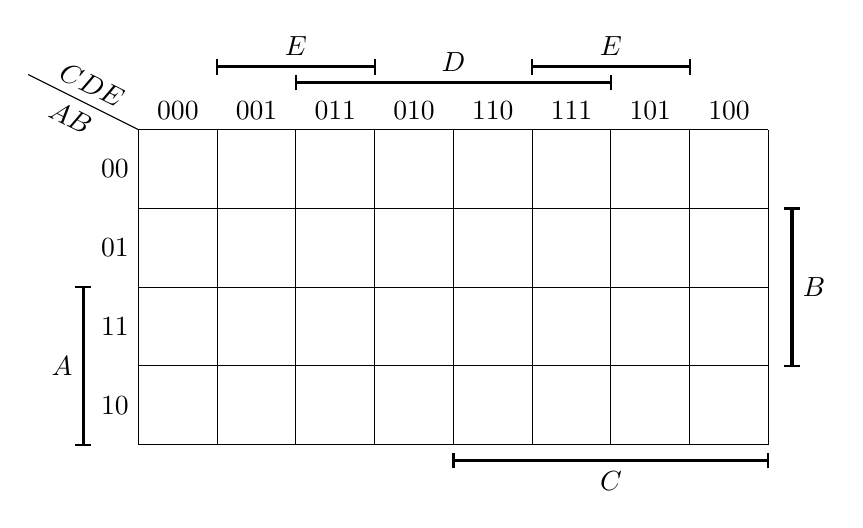
\begin{tikzpicture}[]
            \def\sidelinepaw{0.1}
            \newcommand\sidelineV[4]{% {<start>}{<height>}{<node-style>}{<node-text>}
                \coordinate (start) at #1;
                \draw[thick] (start) +(-\sidelinepaw,0) -- +(\sidelinepaw,0);
                \draw[thick] (start)++(0,#2) +(-\sidelinepaw,0) -- +(\sidelinepaw,0);
                \draw[very thick] (start) -- node[#3]{#4} ++(0,#2);
            }
            \newcommand\sidelineH[4]{% {<start>}{<width>}{<node-style>}{<node-text>}
                \coordinate (start) at #1;
                \draw[thick] (start) +(0,-\sidelinepaw) -- +(0,\sidelinepaw);
                \draw[thick] (start)++(#2,0) +(0,-\sidelinepaw) -- +(0,\sidelinepaw);
                \draw[very thick] (start) -- node[#3]{#4} ++(#2,0);
            }

            \draw (0,0) grid (8,4);
            \node[above] at (0.5,4) {000};
            \node[above] at (1.5,4) {001};
            \node[above] at (2.5,4) {011};
            \node[above] at (3.5,4) {010};
            \node[above] at (4.5,4) {110};
            \node[above] at (5.5,4) {111};
            \node[above] at (6.5,4) {101};
            \node[above] at (7.5,4) {100};
            \node[left] at (0,0.5) {10};
            \node[left] at (0,1.5) {11};
            \node[left] at (0,2.5) {01};
            \node[left] at (0,3.5) {00};
            \draw (0,4) -- node[sloped,below]{$AB$~~} node[sloped,above]{$CDE$} ++(-1.4,.7);

            \sidelineV{(-0.7,0)}{2cm}{left}{$A$}
            \sidelineV{(8.3,1)}{2}{right}{$B$}
            \sidelineH{(4,-0.2)}{4}{below}{$C$}
            \sidelineH{(2,4.6)}{4}{above}{$D$}
            \sidelineH{(1,4.8)}{2}{above}{$E$}
            \sidelineH{(5,4.8)}{2}{above}{$E$}
        \end{tikzpicture}
    \end{subtasks}


    %% Task: Find minimal DNF,CNF,etc using Karnaugh map, and find Zhegalkin polynomial.
    \item For each given function $f_i$ of 4 arguments, draw the Karnaugh map and use it to find BCF, minimal DNF, and minimal CNF\@.
    Additionally, construct ANF (Zhegalkin polynomial) using either the K-map, the tabular (\enquote{triangle}) method or the Pascal method --- use each method at least once.

    \makeatletter
    \newtcolorbox{notebox}[1][]{%
        enhanced jigsaw, % better frame drawing
        borderline west={1pt}{0pt}{black}, % straigh vertical line at the left edge
        sharp corners, % no rounded corners
        boxrule=0pt, % no real frame,
        % fonttitle={\large\bfseries},
        fonttitle={\bfseries},
        coltitle={black},  % Black colour for title
        title={Note},  % Fixed title
        attach title to upper, % Move the title into the box
        after title={:\ },
        colback=gray!10,
        % right=0pt,
        top=0pt,
        bottom=0pt,
        frame hidden,
        baseline={\tcb@height-2\kvtcb@boxsep+\baselineskip-2\lineskip},
        #1
    }
    \makeatother

    \begin{notebox}
        \RaggedRight
        WolframAlpha\Href{https://www.wolframalpha.com} interprets the query \enquote{$n$-th Boolean function of $k$ variables} in a reverse manner.
        In order to employ WolframAlpha properly, manually flip the truth table beforehand, \textit{e.g.} the correct query for $f^{(2)}_{10}$ is \enquote{5th~Boolean function of 2~variables}\Href{https://www.wolframalpha.com/input?i=5th+boolean+function+of+2+variables}, which gives $f^{(2)}_{10} = \neg x_2$, since $\mathtt{rev}(1010_2) = 0101_2 = 5_{10}$.
    \end{notebox}

    \begin{multicols}{2}
    \begin{subtasks}
        \item $f_{\arabic{subtasksi}} = f^{(4)}_{47541}$
        \item $f_{\arabic{subtasksi}} = \sum m (1,4,5,6,8,12,13)$
        \item $f_{\arabic{subtasksi}} = f^{(4)}_{51011} \xor f^{(4)}_{40389}$
        \item $f_{\arabic{subtasksi}} = A\overline{B}D + \overline{A}\,\overline{C}D + \overline{B}C \overline{D} + A\overline{C}D$
    \end{subtasks}
    \end{multicols}


    %% Task: Convert to CNF.
    \item Convert the following formulae to CNF.

    \begin{multicols}{2}
    \begin{subtasks}
        \item $X \iff (A \land B)$
        \item $Z \iff \biglor\nolimits_{i} C_i$
        \item $D_1 \xor \dotsb \xor D_n$
        \item $\operatorname{majority}(X_1, X_2, X_3)$ \footnote{Majority function\Href{https://en.wikipedia.org/wiki/Majority_function} is a Boolean function that is 1 iff the majority (more than half) of the inputs are 1.}
        \item $R \implies (S \implies (T \implies \bigland\nolimits_{i} F_i))$
        \item $M \implies (H \iff \biglor\nolimits_{i} D_i)$
    \end{subtasks}
    \end{multicols}


    %% Task: Functional completeness.
    \item For each given system of functions $F_i$, determine whether it is functionally complete using Post's criterion.
    For each basis $F_i$, use it to represent the $\operatorname{majority}(A,B,C)$ function.
    Draw a combinational Boolean circuit for each resulting formula.

    \begin{multicols}{2}
    \begin{subtasks}
        \item $F_{\arabic{subtasksi}} = \Set{ \land, \lor, \neg }$
        \item $F_{\arabic{subtasksi}} = \Set{ f^{(2)}_{14} }$
        \item $F_{\arabic{subtasksi}} = \Set{ \implies, \centernot\implies }$
        \item $F_{\arabic{subtasksi}} = \Set{ 1, \iff , \land }$
    \end{subtasks}
    \end{multicols}


    %% Task: Prove that Zhegalkin basis is complete.
    \item Show \--- without using Post's criterion \--- that the Zhegalkin basis $\Set{\xor, \land, 1}$ is functionally complete.


    % Task: Truth table for a circuit.
    \item Compute the truth table for the function $f \colon \Bool^3 \to \Bool^2$ (with the semantics $\Triple{A,B,C} \mapsto \Pair{f_{(1)}, f_{(2)}}$) represented with the following circuit.

    \vspace{4pt}
    \begin{circuitikz}[]
        \node (A) at (0,3) {$A$};
        \node (B) at (0,1) {$B$};
        \node (C) at (0,0) {$C$};
        \draw
            (A.east) +(.7,0) coordinate(jA)
            (B.east) +(.7,0) coordinate(jB)
            (C.east) +(2,0) coordinate(jC)

            % g6 = AND(A, g5)
            (A.east) to[short,o-] ++(10,0) node[and port,anchor=in 1](g6){}
            % g3 = NOR(g2, C)
            (C.east) to[short,o-] ++(4,0) node[nor port,anchor=in 2](g3){}
            % g2 = AND(A, B)
            ($(jA)!0.5!(jB)$) ++(1,0) node[and port](g2){}
            % joint after g2
            (g2.out) +(0.5,0) coordinate(jg2)
            % g4 = AND(g2, C)
            (g2.out) -- ++(1.5,0) node[and port,anchor=in 1](g4){}
            % g5 = NOR(g4, g3)
            (g4.out) -- ++(1,0) node[nor port,anchor=in 1](g5){}
            % g1 = OR(A, B)
            (B.east) to[short,o-] ++(10,0) node[or port,anchor=in 2](g1){}
            % g7 = NAND(B, g5)
            (g1) ++ (0,-1) node[nand port](g7){}
            % g8 = NAND(g1, g7)
            (g1.out) -- ++(1,0) node[nand port,anchor=in 1](g8){}

            % joint after g5
            (g5.out) +(0.5,0) coordinate (jg5)
            % joint before g6
            (g6.in 1) +(-0.5,0) coordinate (jg6)
            % joint before g1
            (g1.in 2) +(-0.5,0) coordinate (jg1)

            % outputs
            (g8.out) to[short,-o] ++(0.3,0) node[anchor=west](OUT2){$f_{(2)}$}
            (g6.out) to[short,-o] (g6.out -| OUT2.west) node[anchor=west](OUT1){$f_{(1)}$}

            % interconnections
            (jA) to[short,*-] (jA |- g2.in 1) -- (g2.in 1)
            (jB) to[short,*-] (jB |- g2.in 2) -- (g2.in 2)
            (jg2) to[short,*-] (jg2 |- g3.in 1) -- (g3.in 1)
            (jC) to[short,*-] +(0,0) to[out=90,in=180] (g4.in 2)
            (g3.out) to[out=0,in=180] (g5.in 2)
            (g5.out) to[short,-*] (jg5) to[out=0,in=180] (g6.in 2)
            (jg6) to[short,*-] +(0,0) |- (g1.in 1)
            (jg1) to[short,*-] +(0,0) |- (g7.in 1)
            (jg5) |- (g7.in 2)
            (g7.out) to[out=0,in=180] (g8.in 2)
        ;
    \end{circuitikz}
    % \vspace{6pt}


    %% Task: Binary-to-Gray conversion.
    \item Construct a minimal Boolean circuit that implements the conversion of 4-bit binary numbers to Gray code\Href{https://en.wikipedia.org/wiki/Gray_code}, \textit{i.e.} the function $f \colon \Bool^4 \to \Bool^4$ with the semantics $(b_3,b_2,b_1,b_0) \mapsto (g_3,g_2,g_1,g_0)$, \textit{e\Cat[1.5pt]g.}, $\mathtt{0000}_{2} \mapsto \mathtt{0000}_{\mathrm{Gray}}$, and $\mathtt{1001}_{2} \mapsto \mathtt{1101}_{\mathrm{Gray}}$.
    Use only $\mathtt{NAND}$ and $\mathtt{NOR}$ logic gates.


    % Task: Subtractor.
    \item A \textit{half subtractor} is a circuit that has two bits as input and produces as output a difference bit and a borrow. A \textit{full subtractor} is a circuit that has two bits and a borrow as input, and produces as output a difference bit and a borrow.
    \begin{subtasks}
        \item Construct a circuit for a half subtractor using AND gates, OR gates, and inverters.
        \item Construct a circuit for a full subtractor using half subtractors and NAND gates.
        \item Construct a circuit that computes the \textit{saturating} difference of two four-bit integers $(x_3 x_2 x_1 x_0)_2$ and $(y_3 y_2 y_1 y_0)_2$ using half/full subtractors, AND gates, OR gates, and inverters. When $x \geq y$, the output bits $d_3, \dots, d_0$ should represent $d = x - y$, and when $x < y$, the output must be zero.
    \end{subtasks}


    % Task: Comparator.
    \item Construct a circuit that compares the two-bit integers $(x_1 x_0)_2$ and $(y_1 y_0)_2$, and outputs 1 when $x > y$ and 0 otherwise.


    % Task: Multiplier.
    \item Construct a circuit that computes the product of the two-bit integers $(x_1 x_0)_2$ and $(y_1 y_0)_2$.
    The circuit should have four-bit output $(p_3 p_2 p_1 p_0)_2$ representing the product $ p = x \cdot y$.


    % % Task: MUX.
    % \item A \textit{multiplexer} is a switching circuit that produces as output one of its input bits based on the value of control bits.
    % Construct a 4-to-1 multiplexer (using AND gates, OR gates, and inverters) that has as input the four bits $x_0$, $x_1$, $x_2$, and $x_3$ and the two control bits $c_0$ and $c_1$.
    % The circuit should output~$x_i$, where $i$~is the value of the two-bit integer $(c_1 c_0)_2$.


    %% Task: ITE.
    \item Consider a Boolean function $\operatorname{ITE} \colon \Bool^3 \to \Bool$ defined as follows:
    $\operatorname{ITE}(c,x,y) = \begin{smallcases}
        x & \text{if } c = 0 \\
        y & \text{if } c = 1
    \end{smallcases}$

    Construct a formula for it using the standard Boolean basis $\Set{\land, \lor, \neg}$.
    Determine whether the set $\Set{\operatorname{ITE}}$ is functionally complete.


    %% Task: BDD.
    \item For each given function~$f_i$, construct a Reduced Ordered Binary Decision Diagram (ROBDD) using the natural variable order $x_1 \prec x_2 \prec \dotsb \prec x_n$.
    Determine whether the ROBDD can be reduced even further by using a different variable order \--- if so, show it.

    \begin{defbox}
        Binary Decision Diagram\Href{https://en.wikipedia.org/wiki/Binary_decision_diagram} (BDD) is a representation of a Boolean function as a directed acyclic graph, which consists of \emph{decision} nodes and two \emph{terminal} nodes (0~and~1).
        Each decision node is labeled by a Boolean variable~$x_i$ and has two child nodes called \emph{low} and \emph{high}.
        The edge from node to a low (high) child represents an assignment of the value \texttt{FALSE} (\texttt{TRUE}) to variable~$x_i$.
        A path from the root node to the 1-terminal (0-terminal) corresponds to an assignment for which the represented Boolean function is true (false).

        BDD is called \emph{ordered} if variables appear in the same order on all paths from the root.

        BDD is called \emph{reduced} if it does not contain a node $v$ with $\operatorname{high}(v) = \operatorname{low}(v)$, and there does not exist a pair of nodes $u,v$ such that the sub-OBDDs rooted in $u$ and $v$ are isomorphic.
    \end{defbox}

    \begin{multicols}{2}
    \begin{subtasks}
        \item $f_{\arabic{subtasksi}}(x_1,\dots,x_4) = x_1 \xor x_2 \xor x_3 \xor x_4$
        \item $f_{\arabic{subtasksi}}(x_1,\dots,x_5) = \operatorname{majority}(x_1,\dotsc,x_5)$
        \item $f_{\arabic{subtasksi}}(x_1,\dots,x_4) = \sum m(1,2,5,12,15)$
        \item $f_{\arabic{subtasksi}}(x_1,\dots,x_6) = x_1 x_4 + x_2 x_5 + x_3 x_6$
    \end{subtasks}
    \end{multicols}

    % \item \ldots
\end{tasks}

\end{document}
